\chapter{Measurement Results}\label{ch:results}
\section{Measurement Setup}
Fig. \ref{fig:setup} shows the measurement setup of a split cylinder resonator prototype that we developed and used for our measurements. In our setup the cylindrical cavities of the resonator were placed in a v-shaped groove of a hard wood base. The groove was clad with an aluminium sheet to avoid wear of the wooden base. Unlike other split cylinder resonator setups, our arrangement was self-aligning, which greatly simplified the setup. To provide enough room for large sheet samples we cut a slot into the base, in which large specimen may be inserted. A simple clamp mechanism was also added, which allowed us to firmly clamp the sample between the two cavities.

The cavities themselves were manufactured on a general purpose lathe from leaded brass (CuZnPb3). The blind holes of the cavities were first drilled, then the openings were enlarged using a boring bar. The face of the cavities, which are the flanges of the resonator, were also shaped in the same step to ensure proper alignment. The surface roughness of the cuts was note refined by any additional process like surface grinding or lapping. Generally speaking, a good surface finish guarantees high quality factors of the resonances, since a rough surface will have a higher surface impedance. High quality factors are essential for dielectric measurements with resonators, because resonances with a high quality factor have a narrow bandwidth and will therefore be less likely disturbed by neighbouring modes. In the light of this fact one might argue that lead brass with its relatively low bulk conductivity of \SI{15}{\mega\siemens\per\meter} is a bad choice as material for the cavities, since the conductivity is far lower than that of copper (\SI{58}{\mega\siemens\per\meter}) or silver (\SI{63}{\mega\siemens\per\meter}). It is widely noted that brass is still an excellent choice as material for cavities, because it is easily machinable and can be electroplated with better conductors to improve its conductivity. Still, we do not gain much from a better conductor on the cavity walls, since the quality factor is only proportional to the square root of the conductivity, $Q\propto\sqrt{\sigma}$. We measured a surface conductivity of around \SI{10}{\mega\siemens\per\meter} for our cavities, if we changed the material for the best conductor available, which is silver with a bulk conductivity of \SI{63}{\mega\siemens\per\meter}, the quality factor would increase less than two and a half fold.
\begin{equation*}
\frac{Q_\text{Silver}}{Q_\text{Brass,m}}\leq\sqrt{\frac{63}{10}}=2.45
\end{equation*}
Of course, this also means that the bandwidth of the resonance would decrease less than two and a half fold, which shows that the potential gain in accuracy is limited. If the amount of dielectric loss in a measurement is high, the gain will be even smaller. Finishing processes like diamond turning or grinding may still be beneficial for the performance of a cavity, since these processes typically have a higher manufacturing accuracy. Higher manufacturing accuracy also means lower uncertainty for the geometry of the apparatus, which in turn can increase the accuracy of dielectric measurements.

\begin{figure}
\centering
\begin{tikzpicture}
%\draw[step=0.25cm,gray,very thin] (-2,0) grid (13,7);
    \node[anchor=south west,inner sep=0] (image) at (0,0) {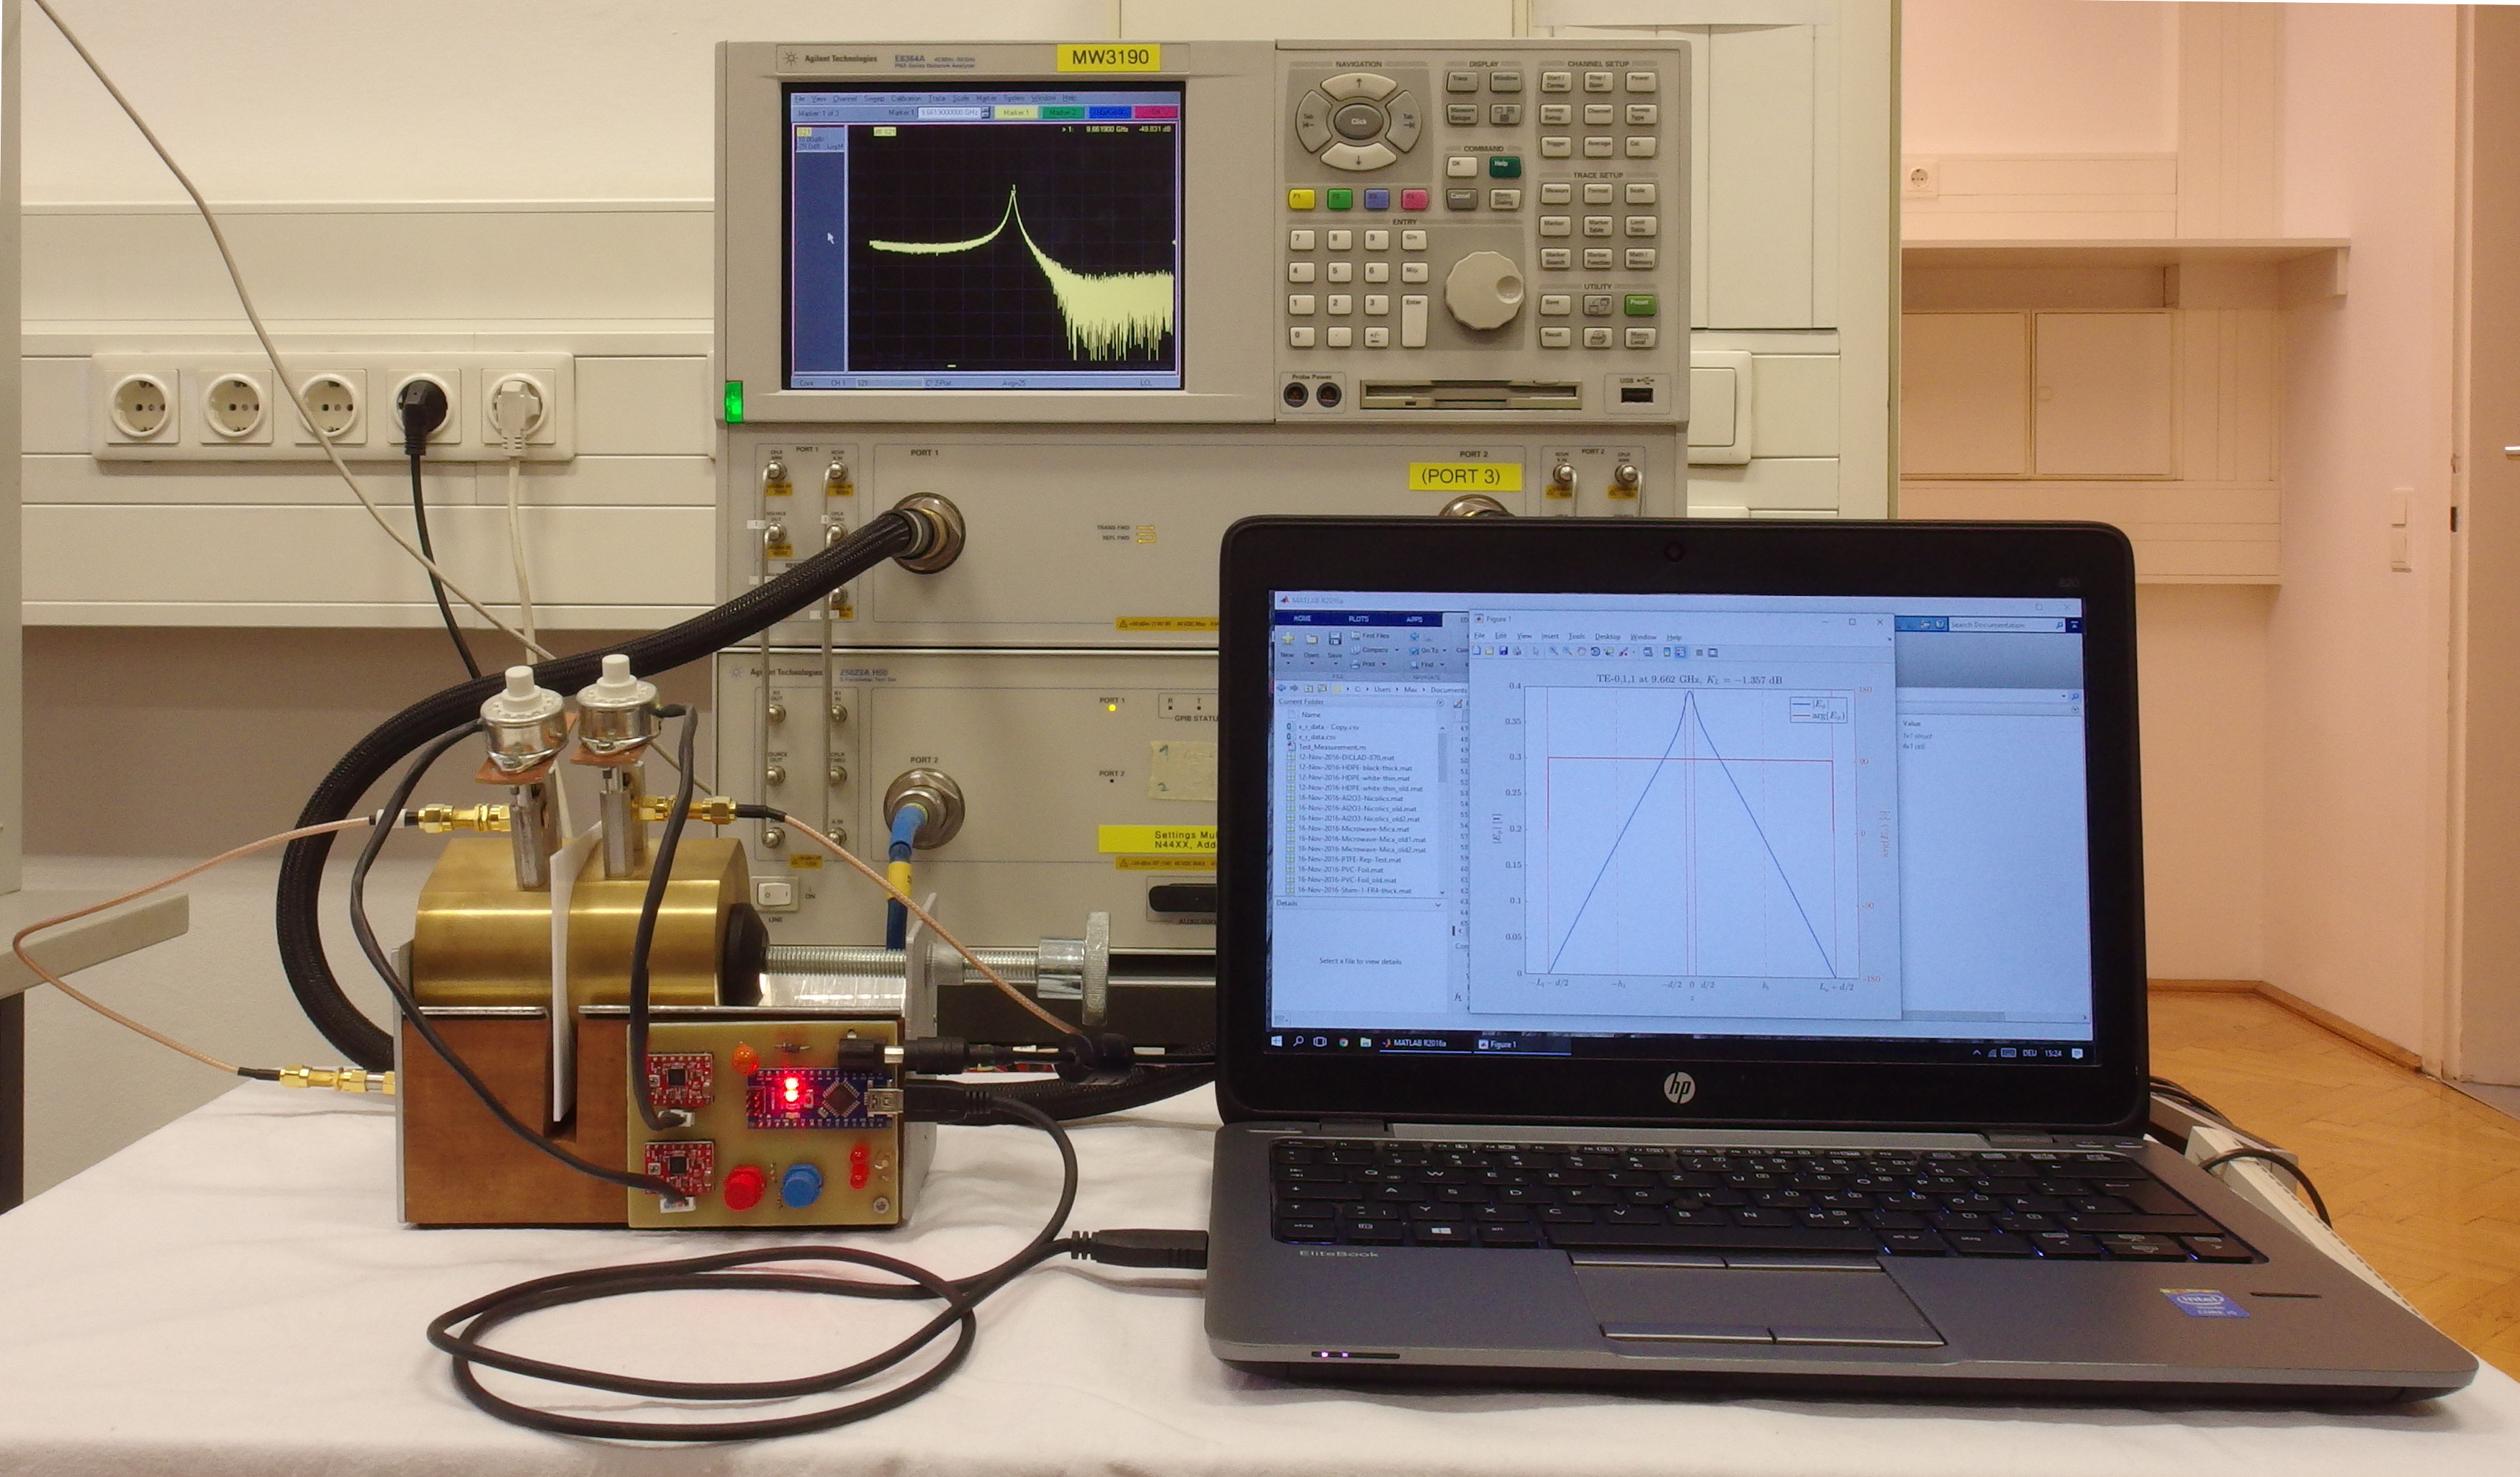
\includegraphics[height=6.45cm]{Measurement_setup_cropped.jpg}};
    
    \draw [-latex, thick, red] (-0.25,2.25) node[anchor=east, black,text width=2cm,align=right] {Resonator} to (1.8,2.25);
    \draw [-latex, thick, red] (-0.25,5.5) node[anchor=east, black,text width=2cm,align=right] {Coupling adjustment mechanisms} to (2.15,3.35);
    \draw [-latex, thick, red] (-0.25,5.5) to (2.65,3.625);    
    \draw [-latex, thick, red] (-0.25,0.75) node[anchor=east, black,text width=2cm,align=right] {PTFE sample} to (2.43,1.75);
    \draw [-latex, thick, red] (-0.25,3.75) node[anchor=east, black,text width=2cm,align=right] {Coaxial lines} to (0.8,2.65);
    \draw [-latex, thick, red] (-0.25,3.75) to (4,2.5);
    
    \draw [-latex, thick, red] (11.22,5.5) node[anchor=west, black,text width=2cm,align=left] {VNA} to (7.4,5);
    \draw [-latex, thick, red] (11.22,3.25) node[anchor=west, black,text width=2cm,align=left] {PC} to (9.4,3);    
    \draw [-latex, thick, red] (11.22,1) node[anchor=west, black,text width=2cm,align=left] {USB cable} to (4.25,0.5);

\end{tikzpicture}
\caption{Photograph of the measurement setup.}\label{fig:setup}
\end{figure}

The cavities were coupled to a vector network analyser by means of magnetic coupling loops, which were inserted into holes drilled into the cavities. The coupling loops were made from RG405 semi-rigid coaxial cable by soldering the inner conductor onto the outer conductor. To make the coupling adjustable we developed an electronic coupling adjustment mechanism. This mechanism works as such that the coupling loops are mounted on the shanks of two linear stepper motors. When the stepper motors extend the shanks, the coupling loops are lowered into the cavities and the coupling increases. Conversely, when the shanks are pulled up by the stepper motors, the loops are moved out of the cavity and the coupling decreases. The two stepper motors were driven by an electronic circuit, which could be remote controlled from a PC. The interface with a PC allowed the measurement software to adjust the coupling of the resonator, which was especially useful for broadband measurements. In a cavity the coupling coefficients vary from mode to mode, so the coupling needs to be adjusted for every mode to keep the coupling coefficient at the desired level. The electronic adjustment mechanism simplifies the measurement procedure and speeds up the measurement compared to a manual adjustment mechanism. Additionally, the stepper motors we used had a linear travel per step of only \SI{1}{thou} (\SI{25,4}{\micro\meter}), which also allowed to us to adjust the coupling more precisely. Besides allowing us to fine-tune the coupling, the stepper motors also made it possible to adjust the coupling symmetrically and keep the symmetry while adjusting the coupling. As we have discussed previously, symmetric coupling allows us to determine the coupling coefficient from the maximum of the transmission coefficient. The coupling coefficient of a very under-coupled resonator is almost negligible, but symmetric coupling may be used to improve the accuracy of our quality factor measurements.

The measurement results were computed with a measurement software written in the MATLAB scripting language. It was designed by us as a software suite for calibrations and measurements with a split cylinder resonator. The software was run by a PC next to the vector network analyser (VNA), which was connected to the VNA through an ethernet connection and to the coupling adjustment circuit through a USB connection. A wide range of different features of the software were used in our measurements. The software set up the transmission coefficient measurements on the VNA, fetched the measurement data and saved it on the PC for later use. It also determined the resonances of the frequency response of the transmission coefficient and adjusted the coupling appropriately through the electronic adjustment mechanism. From the measured resonance curves it determined the quality factor and the resonant frequency of the resonance. The software supported a wide range of different quality factor measurement techniques like the 3dB method, the Coakley method and a circle-fit. The measurement results of the quality factor measurements were then used by the software to compute the relative permittivity and the loss tangent for the TE\st{011} modes as well as higher modes. Or, if the software was in calibration mode, it was used to calculate the calibration radius $a_l$ and the conductivity $\sigma$. If the calibration data was used in a measurement, the software allowed the operator to use different calibrations for different modes (broadband calibration). The software supported both the Janezic model and our very own M12 model. Finally, if the resonant frequency of the TE\st{011} mode or any other higher TE\st{0np} mode was unknown, the software had a feature to estimate the permittivity from the fundamental mode. This estimate could then be used to estimate the resonant frequency of the mode in question.
\section{Measurement Flow}
\begin{figure}
\centering
% Define block styles
\tikzstyle{block} = [rectangle, draw, fill=blue!20, 
    text width=6.3em, text centered, rounded corners, minimum height=3.5em]
\tikzstyle{line} = [draw, -latex',font=\fontsize{9}{9}]
    
\begin{tikzpicture}
    % Place nodes
    \node [block] (empty_res) {Empty resonator characterisation};
    \node [block, below of=empty_res, node distance=2cm] (cal) {Calibration};        
    \node [block, right of=cal, node distance=3.7cm] (esti) {TE\st{0np} resonant frequency estimation};
    \node [block, below of=esti,node distance=2cm] (meas) {Transmission coefficient measurement};
    \node [block, right of=esti, node distance=3.5cm] (eresti) {Relative permittivity estimation};
    \node [block, left of=cal, node distance=4.2cm] (length) {Resonator dimensions measurement};
    \node [block, below of=meas, node distance=2cm] (calc) {$\varepsilon_r$ and $\tan\delta$ calculation};
    \node [block, above of=esti, node distance=2cm] (thickness) {Sample thickness measurement};
    \node [block, below of=calc, node distance=2cm] (uncert) {Uncertainty estimation};
    \node [coordinate, below of=uncert, node distance=1.2cm] (bert) {Uncertainty estimation};
    % Draw edges
    \draw[dashed] (1.85,0.5) -- (1.85,-9.5);
    \path [line] (empty_res) -- node[anchor=east] {$f_\text{r,empty}$, $Q_\text{0,empty}$} (cal);
    \path [line] (cal) -- node[anchor=south] {$a_l, \sigma$} (esti);
    \path [line] (esti) -- node[anchor=west] {$f_{r,\text{est}}$} (meas);
    \path [line] (eresti) -- node[anchor=south] {$\epsilon_{r,\text{est}}$} (esti);
    \path [line] (meas) -- node[anchor=west] {$f_r, Q_0$} (calc);
    \path [line] (calc) -- node[anchor=west] {$\epsilon_r,\tan\delta$} (uncert);
    \path [line] (thickness) -- node[anchor=west] {$d$} (esti);
    \path [line] (length) -- node[anchor=south] {$L_l$, $L_u$, $a_u$} (cal);
    \path [line] (uncert) -- (bert) node[anchor=north] {$u(\varepsilon_r),u(\tan\delta)$};
\end{tikzpicture}
\caption{Flow diagram of a measurement with the M12 model.}\label{fig:flow}
\end{figure}

The flow diagram shown in Fig. \ref{fig:flow} illustrates the individual steps of a measurement with the M12 model. Although we have already discussed many aspects of the measurement like the theory of the model, the calibration of the resonator or quality factor measurements of resonance curves, it is  still worthwhile to take a closer look at the measurement process and to explain how the different steps of a measurement interact. When we take a look at the measurement shown in the flow diagram, the first thing that strikes us is the dashed line in the middle of the diagram.  This line divides the measurement process into two procedures, the calibration procedure on the left hand side and the measurement procedure on the right hand side. The blocks shown in the diagram are the step of these two procedures and the lines connecting the blocks are the variables that are determined in the step they originate from. The line crossing the dashed line separating the two procedures carries along the calibration variables from the calibration to the measurement procedure and connects the two procedures.

In the calibration procedure one of the first steps is the measurement of the resonator dimensions, which determines the lengths of the cavities $L_u$ and $L_l$, and the radius of the upper cavity $a_u$. Both should be measured accurately with a calliper or a micrometer. In the next step, the empty resonator characterisation, the cavities are pressed together to form a cylindrical cavity, and the resonant frequencies and quality factors of the resonant modes of the cavity are measured. These and the resonator dimension are then handed over to the last step in the calibration, which calculates the radius of the lower cavity $a_l$ and conductivity $\sigma$ for each of the calibration modes.

This step ends the calibration and delivers the calibration parameters to the measurement procedure. The first step in the measurement procedure is the estimation of the resonant frequencies of the TE\st{0np} modes. As this step uses the M12 model to estimate the resonant frequencies, all dimensions of the resonator are required. Out of this reason the thickness of the sample needs to be measured, for example with a micrometer. Apart from the sample thickness measurement, which gives the thickness $d$ of the specimen, estimating the resonant frequencies of the modes also requires an estimate for the relative permittivity of the specimen $\epsilon_{r,est}$. This relative permittivity of the specimen can be estimated, for example, from a value in a data sheet or from a measurement of the fundamental TE\st{111} mode of the split cylinder resonator. With these two parameters the resonant frequencies are estimated and passed on to the next step, the transmission coefficient measurement. In this step the sample is inserted into the resonator and the transmission coefficient is measured around the estimated resonant frequencies. If there is no overlap with other modes, this measurement yields the resonance curves of the TE\st{0np} modes. These curves are then used to calculate the resonant frequencies $f_r$ and quality factors $Q_0$ of the modes. Finally, this brings to the most interesting step of the measurement, the calculation of the relative permittivity and loss tangent of the sample. In this step the relative permittivity and the loss tangent of the sample are calculated from the resonator dimensions, the resonant frequencies and the quality factors of the modes using the M12 model. This calculation yields the results of the measurement. Lastly, the uncertainty of the measurement can be estimated, if multiple measurements of the specimen and the calibration are performed. 
\section{Uncertainty Budget of the M12 Matrix Model}
%%%%%%%%%%%%%%%%%%%%%%%%%%%%%% UNCERTAINTY BUDGET COMMAND %%%%%%%%%%%%%%%%%%%%%%%%%%%%%%%%%%%%%
\newcolumntype{C}[1]{>{\centering\let\newline\\\arraybackslash\hspace{0pt}}m{#1}}
\newcommand{\uncertbl}[2]{
\pgfplotstabletypeset[sci zerofill,precision=2,font=\scriptsize,
					  col sep=tab,
                      every head row/.style={before row=\hline\rule{0pt}{2.6ex}
										     #1 & \multicolumn{7}{c|}{ }\\\hline\rowcolor{gray!20}\rule{0pt}{2.6ex},after row=\hline\rule{0pt}{2.6ex}},
					  columns={symb,sourceu,value,unit,pdf,div,coeff,ui},
                      every last row/.style={after row=\hline},
                      columns/symb/.style={column type=|C{0.06\textwidth},column name=Symb.,string type},
                      columns/sourceu/.style={column type=|C{0.18\textwidth},column name={Source of uncertainty},string type},	
					  columns/value/.style={column type=|C{0.09\textwidth},column name={Value $\pm$}},
					  columns/unit/.style={column type=C{0.04\textwidth},column name={Unit},string type},
					  columns/pdf/.style={column type=|C{0.16\textwidth},column name={Probability dist.},string type},		
         		      columns/div/.style={column type=|C{0.03\textwidth},column name={Div.},string type},
					  columns/coeff/.style={column type=|C{0.09\textwidth},column name={$c_i$}},
					  columns/ui/.style={column type=|C{0.09\textwidth}|,column name={$u_i$}},
                      %columns/vi/.style={column type=|C{0.05\textwidth}|,column name={$\nu_i$},string type},
                      empty cells with={ },
						]#2}
%%%%%%%%%%%%%%%%%%%%%%%%%%%%%%%%%%%%%%%%%%%%%%%%%%%%%%%%%%%%%%%%%%%%%%%%%%%%%%%%%%%%%%%%%%%%%%%%%
This section deals with the uncertainty of a measurement with the M12 model and compares it to the uncertainty of measurements with the Janezic model. In the title of this thesis we emphasised that this model is an improved model for complex permittivity measurements with a split-cylinder resonator. Our model is in principle an expansion of the Janezic model and also uses mode-matching to solve the field problem. Still, our model solves the field problem for a cavity with unequal half-cavities, which eliminates the systematic error of the symmetric model. As we will see later in this section, this can reduce the uncertainty of a relative permittivity measurement by more than 70\% and, hardly noticeable, that of loss tangent measurements by around 5\%. 

To illustrate the improvements in accuracy we have calculated the uncertainty budget of a measurement. For this measurement we measured the same PTFE sample that we have used for most of our previous examples. The measurements were performed with \te{} modes at a constant ambient temperature of around \SI{22}{\celsius}. The calculation of the uncertainty budget included Type A and Type B uncertainties, where Type A refers to uncertainties evaluated by a statistical analysis of a series of observations and Type B roughly refers to systematic uncertainties. An in-detail explanation of these two kinds of uncertainties can be found in a guide published by UKAS \cite{UKAS} and in the GUM \cite{GUM}. The Type A uncertainties were evaluated in a repeatability evaluation (Sec. \ref{sec:rep}) of the calibration and of the complex permittivity measurement. With respect to the statistical analysis of the measurement values, we decided to report all expanded uncertainties for a coverage probability of close to 95\%, which required a coverage factor of around 2 for a Gaussian distribution. Unlike many other researchers, our evaluations were performed under a worst-case assumption, and hence we used uniform distributions for all inputs with a unknown probability distribution. Since the probability distribution and the coverage of random variables with input variables that have a uniform distribution is not Gaussian, we used a Monte-Carlo simulation (NIST uncertainty machine) to compute the probability distributions and coverage factors for all variables.

The quality factor and resonant frequency of the measurement modes were obtained from transmission coefficient measurements with a Keysight PNA E8364A vector network analyser. The VNA was calibrated at a right-angle SMA connector that connected the coupling loops to the coaxial lines of the VNA. The calibration was performed with a Keysight N4433A electronic calibration module, which also limited the frequency range of our measurements to less than \SI{20}{\giga\hertz}. To ensure good linear performance and high dynamic range the output power of the VNA was set to \SI{0}{dBm}, which improved the measurement accuracy for small transmission coefficients in the \SIrange{-70}{-50}{\decibel} range. Each measurement was an average over 25 measurement sweeps, which were measured with the default IF bandwidth of \SI{35}{\kilo\hertz}. For this configuration we estimated the accuracy of the transmission coefficient measurement using the Keysight VNA uncertainty calculator. The calculator estimated an accuracy of less than \SI{0.93}{\decibel} for the magnitude and an accuracy of less than \SI{6.5}{\degree} for the phase in the \SIrange{-70}{-50}{\decibel} range. Using these accurate transmission coefficient measurements we were able to measure the quality factor and the resonant frequency very accurately. We evaluated the uncertainty of the quality factor measurements using the findings of Petersan and Anlage \cite{petersan}, see Sec. \ref{sec:rescurve}. The quality factors and resonant frequencies were measured using a circle-fit of the measured resonance curves. All resonance curves of the calibration and of the permittivity measurements had SNRs (for a definition of this SNR, please refer to \cite{petersan}) exceeding 60. Petersan and Anlage found that the relative accuracy of a circle-fit, which is more or less identical to the phase vs. frequency fit discussed in their article, for such high SNRs and a quality factor of around \num{e3} was less than \num{7.88e-8} for the resonant frequency and less than \num{1.3e-4} for the quality factor. Although the relative precision of the quality factor was lower than the accuracy of the method, we evaluated the uncertainty of the quality factor measurements using only the relative accuracy. This was acceptable as the quality factor measurements were found to have a negligible influence on our calibration parameters and on our permittivity measurements. For lower SNRs a more accurate analysis should be performed. 

\subsection{Uncertainty of Dimensional Measurements}
\begin{table}[ht]
\centering
%%% UNCERTAINTY OF L						
\pgfplotstableread[col sep=tab]{
symb	sourceu	value	unit	pdf	div	coeff	ui	vi
u\st{r}	Flatness	3.70E-05	m	Uniform	$\sqrt{3}$	1	2.14E-05	∞
u\st{m}	Calliper	2.11E-05	m	Uniform	$\sqrt{3}$	1	1.22E-05	∞
u(L)	Combined uncertainty		m	Convolved			2.46E-05	∞
U	Expanded uncertainty		m	Convolved (k=1.9)			4.67E-05	∞
}\uncertl
\uncertbl{$L$}{\uncertl}
\caption{Uncertainty budget of $L$ of the Janezic model.}\label{u:L}
\end{table}

Starting point for any measurement with a split-cylinder resonator are dimensional measurements of the resonator. In the \textbf{Janezic model} the only dimension that had to be measured is the length $L$ of the cavities. The cavity length $L$ was measured with a digital calliper along the circumference of the bore. Each cavity was measured 20 times. The dimensional uncertainty of $L$ was evaluated using a uniform distribution, which used the sample mean of these measurements as mean $\mu_L$ and the largest difference $u_r=\Delta_L$ of a measurement value from the sample mean as half-width of the uniform distribution:
\begin{equation}
f_L(L)=\begin{cases}\frac{1}{2\Delta_L}, & \mu_L-\Delta_L\leq L\leq \mu_L+\Delta_L\\
					0, & \text{elsewhere} \\
	    \end{cases}
\end{equation}
We used the uniform distribution in line with our worst-case assumption for the evaluation of uncertainty. The expanded uncertainty of the depth measurements at a coverage probability of 95\% was $\text{MPE}_E+\text{MPE}_S=\SI{40}{\micro\meter}$ in accordance with DIN862. Similar to the dimensional uncertainty, the uncertainty of depth measurements was evaluated using a uniform distribution with $u_m=\frac{1}{0.95}(\text{MPE}_E+\text{MPE}_S)=\SI{42.1}{\micro\meter}$. The uncertainty budget of $L$ is shown in Table \ref{u:L}.

\begin{table}[ht]
\centering

%%% UNCERTAINTY OF L_U						
\pgfplotstableread[col sep=tab]{
symb	sourceu	value	unit	pdf	div	coeff	ui	vi
u\st{r}	Flatness	9.00E-06	m	Uniform	$\sqrt{3}$	1	5.20E-06	∞
u\st{m}	Calliper	2.11E-05	m	Uniform	$\sqrt{3}$	1	1.22E-05	∞
u($L_u$)	Combined uncertainty		m	Convolved			1.32E-05	∞
U	Expanded uncertainty		m	Convolved (k=1.8)			2.38E-05	∞
}\uncertlu
\uncertbl{$L_u$}{\uncertlu}

\vspace{7px}

%%% UNCERTAINTY OF L_L						
\pgfplotstableread[col sep=tab]{
symb	sourceu	value	unit	pdf	div	coeff	ui	vi
u\st{r}	Flatness	2.30E-05	m	Uniform	$\sqrt{3}$	1	1.33E-05	∞
u\st{m}	Calliper	2.11E-05	m	Uniform	$\sqrt{3}$	1	1.22E-05	∞
u(L\st{l})	Combined uncertainty		m	Convolved			1.80E-05	∞
U	Expanded uncertainty		m	Convolved (k=1.9)			3.42E-05	∞
}\uncertll
\uncertbl{$L_l$}{\uncertll}

\vspace{7px}

%%% UNCERTAINTY OF A_U
\pgfplotstableread[col sep=tab]{
symb	sourceu	value	unit	pdf	div	coeff	ui	vi
{u\st{taper}}	Taper	4.62E-06	m	Uniform	$\sqrt{3}$	1	2.67E-06	∞
{u\st{m}}	Inside Micrometer	2.11E-06	m	Uniform	$\sqrt{3}$	1	1.22E-06	∞
u($a_u$)	Combined uncertainty		m	Convolved			2.93E-06	∞
U	Expanded uncertainty		m	Convolved (k=1.8)			5.28E-06	∞
}\uncertau
\uncertbl{$a_u$}{\uncertau}
\caption{Uncertainty budget of $a_u$, $L_u$ and $L_l$ of the M12 model.}\label{u:Ll}
\end{table}

For the \textbf{M12 model} the situation was a bit more complicated, because the radius of the upper cavity $a_u$, the length of the lower cavity $L_l$ and the length of the upper cavity $L_u$ had to be measured. The radius $a_u$ was measured ten times at three different depths of the bore using a bore gauge. As probability distribution a uniform distribution was chosen for the radius, which used the sample mean as mean value and the largest deviation of a measurement value from the mean as half-width of the distribution. The gauge had an expand uncertainty for the diameter of \SI{4}{\micro\meter} in accordance with DIN863-4. The lengths of the cavities were measured in the same way as for the Janezic model, only the uncertainty was evaluated individually for each cavity. The uncertainty budgets of $a_u$, $L_l$ and $L_u$ are shown in Table \ref{u:Ll}.

\begin{table}[ht]
\centering
%%% UNCERTAINTY OF D
\pgfplotstableread[col sep=tab]{
symb	sourceu	value	unit	pdf	div	coeff	ui	vi
{u\st{flat}}	Flatness	3.85E-06	m	Uniform	$\sqrt{3}$	1	2.22E-06	∞
{u\st{m}}	Micrometer	4.21E-06	m	Uniform	$\sqrt{3}$	1	2.43E-06	∞
u(d)	Combined uncertainty		m	Convolved			3.29E-06	∞
U	Expanded uncertainty		m	Convolved (k=1.9)			6.26E-06	∞
}\uncertd
\uncertbl{$d$}{\uncertd}
\caption{Uncertainty budget of $d$.}\label{u:d}
\end{table}

The \textbf{thickness $\mathbf{d}$} of the Janezic model and of the M12 model were identical, likewise the uncertainties were evaluated in the same way. The thickness of the PTFE sample was measured twenty times - each time at a different location on the sample - using an outside micrometer. We used the sample mean as the mean of $d$, and the largest deviation of a measurement value $u_\text{flat}=\Delta_d$ from the mean as the error due to thickness variations of the sample. In line with our worst-case assumption the error had a uniform distribution. The measurements were performed with a digital outside micrometer, which was put in a small vice to avoid measurement errors due to thermal expansion of the micrometer frame. The micrometer had an expanded uncertainty (MPE) of \SI{4}{\micro\meter} according to DIN863-1. The measurement error of the micrometer was modelled with a uniform distribution, which had a half-width of $u_m=\frac{1}{0.95}\text{MPE}=\SI{4.21}{\micro\meter}$. The uncertainty budget of $d$ is shown in Table \ref{u:d} and all dimensions and the thickness of the sample are listed in Table \ref{u:dim}. 

\begin{table}[ht]
\centering
\scriptsize
\newcolumntype{P}{>{\centering\arraybackslash}p{0.125\textwidth}}
\begin{tabular}{|P|P|P|P|P|P|}
\hline \rule{0pt}{2.6ex}
 & $\mathbf{L}$ & $\mathbf{L_u}$ & $\mathbf{L_l}$ & $\mathbf{a_u}$ & $\mathbf{d}$ \\ 
\hline \rule{0pt}{2.6ex}
Mean $\mu$ & \SI{25.023}{\milli\meter} & \SI{25.009}{\milli\meter} & \SI{25.037}{\milli\meter} & \SI{19.09}{\milli\meter} & \SI{1.5092}{\milli\meter} \\ 
\hline \rule{0pt}{2.6ex}
Half-width $\pm\Delta$ & \SI{37}{\micro\meter} & \SI{9}{\micro\meter} & \SI{23}{\micro\meter} & \SI{4.62}{\micro\meter}  & \SI{3.85}{\micro\meter}  \\ 
\hline \rule{0pt}{2.6ex}
Measurement & $20\times$ along perimeter of each cavity & 20x along perimeter & 20x along perimeter & 10x at three depth levels & 20x at various locations on sample \\ 
\hline \rule{0pt}{2.6ex}
Instrument & Calliper & Calliper & Calliper & Bore gauge & Outside micrometer \\ 
\hline
\end{tabular} 
\caption{Dimensions of the split-cylinder prototype and thickness of the sample.}\label{u:dim}
\end{table}

\subsection{Uncertainty of Permittivity Measurements}

\begin{table}
\centering
%%% UNCERTAINTY OF A CAL						
\pgfplotstableread[col sep=tab]{
symb	sourceu	value	unit	pdf	div	coeff	ui
f\st{r,cal}	Resonant frequency	7.91E+02	Hz	Normal	1	2.09E-12	1.65E-09
L	Cavity length	6.15E-05	m	Convolved (k=1.9)	1.9	7.44E-02	2.41E-06
{$\Delta$}	Difference from dimensional measurement	3.27E-05	m	Convolved (k=1.6)	1.6	1	2.04E-05
a\st{r}	Repeatability	8.49E-07	m	Normal	1	1	8.49E-07
u(a)	Combined standard uncertainty			Quasi-Normal			2.06E-05
U	Expanded uncertainty			Quasi-Normal (k=2)			4.03E-05
}\uncertja
\uncertbl{$a$}{\uncertja}

\vspace{7px}

%%% UNCERTAINTY OF SIGMA CAL						
\pgfplotstableread[col sep=tab]{
symb	sourceu	value	unit	pdf	div	coeff	ui
f\st{r,cal}	Resonant frequency	7.91E+02	Hz	Normal	1	1.00E-03	7.92E-01
Q\st{cal}	Quality factor	1.60	-	Normal	1	1.63E+03	2.61E+03
a	Cavity radius	4.03E-05	m	Quasi-Normal (k=2)	2	6.23E+07	1.26E+03
L	Cavity length	6.15E-05	m	Convolved (k=1.9)	1.9	4.75E+07	1.54E+03
σ\st{r}	Repeatability	2.23E+05	S/m	Normal	1	1	2.23E+05
u(σ)	Combined standard uncertainty			Quasi-Normal			2.23E+05
U	Expanded uncertainty			Quasi-Normal (k=2)			4.38E+05
}\uncertjsigma
\uncertbl{σ}{\uncertjsigma}
\caption{Uncertainty budget of $a$ and $\sigma$ of the Janezic calibration.}\label{u:cal_j}
\end{table}

Using the uncertainty budget of the dimensional measurements and the findings of Petersan and Anlage \cite{petersan}, we calculated the uncertainty budget of the calibration parameters and of the measurement results for the Janezic model and for the M12 model. In the uncertainty calculation all input variables were assumed to be independent random variables. To simplify the calculations correlations between the calibration parameters and the resonator dimensions were ignored. Computations including the correlations showed that these changed the results very little. Apart from that, the upper limit on the uncertainty guaranteed an uncertainty of less than the sum of all uncertainties, as stated by Taylor \cite[Sec. 9.2]{taylor}. 

We started the calculations by first determining the sensitivity coefficients $c_i$ of each model. These coefficients were computed with our measurement software and $N=75$ modes were included in each of the calculations. The coefficients for the uncertainty budget of the calibration were determined for a resonant frequency of $f_r=\SI{10.040}{\giga\hertz}$ and a quality factor of $Q=\num{12299}$. And, the coefficients for the uncertainty budget of the measurement were computed for a resonant frequency of $f_r=\SI{9.6619}{\giga\hertz}$, a quality factor of $Q=\num{8882}$, a thickness of the sample of $d=\SI{1.509}{\milli\meter}$ and a sample radius of $b=\SI{35}{\milli\meter}$. 

Secondly, we performed calibration measurements of the empty resonator and permittivity measurements of the PTFE sample 20 times to study the repeatability of each measurement. In these measurements, we rotated the cavities after each measurement, so that the orientation of the two half-cavities changed from measurement to measurement. This was done to account for the random error caused by the misalignment of the cavities in the mount. Before we conducted this repeatability evaluation, we first cleaned the resonator with soap to remove any dirt left by machining, then we cleaned resonator and sample with Isopropyl alcohol. After the cleaning we dried both of them thoroughly. 

\begin{table}
\centering
%%% UNCERTAINTY OF A_L CAL					
\pgfplotstableread[col sep=tab]{
symb	sourceu	value	unit	pdf	div	coeff	ui
f\st{r,cal}	Resonant frequency	7.91E+02	Hz	Normal	1	4.16E-12	3.29E-09
a\st{u}	Upper cavity radius	5.28E-06	m	Convolved (k=1.8)	1.8	9.95E-01	2.92E-06
L\st{u}	Upper cavity length	4.47E-05	m	Convolved (k=1.8)	1.8	7.31E-02	1.82E-06
L\st{l}	Lower cavity length	5.26E-05	m	Convolved (k=1.9)	1.9	7.57E-02	2.10E-06
{$\Delta$}	Difference from dim. measurement	1.44E-05	m	Convolved (k=1.7)	1.7	1	8.45E-06
a\st{l,r}	Repeatability	1.72E-06	m	Normal	1	1	1.72E-06
u(a\st{l})	Combined standard uncertainty			Quasi-Normal			9.51862E-06
U	Expanded uncertainty			Quasi-Normal (k=1.9)			1.80854E-05
}\uncertmal
\uncertbl{$a_l$}{\uncertmal}

\vspace{7px}

%%% UNCERTAINTY OF SIGMA CAL					
\pgfplotstableread[col sep=tab]{
symb	sourceu	value	unit	pdf	div	coeff	ui
f\st{r, cal}	Resonant frequency	7.91E+02	Hz	Normal	1	5.01E-03	3.96E+00
Q\st{cal}	Quality factor	1.60E+00	-	Normal	1	1.63E+03	2.61E+03
a\st{u}	Upper cavity radius	5.28E-06	m	Convolved (k=1.8)	1.8	4.98E+08	1.46E+03
a\st{l}	Lower cavity radius	1.81E-05	m	Quasi-Normal (k=1.9)	1.9	4.83E+08	4.60E+03
L\st{u}	Upper cavity length	4.47E-05	m	Convolved (k=1.8)	1.8	2.66E+08	6.62E+03
L\st{l}	Lower cavity length	5.26E-05	m	Convolved (k=1.9)	1.9	1.82E+08	5.03E+03
σ\st{r}	Repeatability	2.24E+05	S/m	Normal	1	1	2.24E+05
u(σ)	Combined standard uncertainty			Quasi-Normal			2.25E+05
U	Expanded uncertainty			Quasi-Normal (k=2)			4.40E+05
}\uncertmsigma
\uncertbl{σ}{\uncertmsigma}
\caption{Uncertainty budget of $a_l$ and $\sigma$ of the M12 calibration.}\label{u:cal_m12}
\end{table}

Tables \ref{u:cal_j} and \ref{u:cal_m12} show our results for the calibration parameters. In the case of the Janezic model these parameters were the radius of the cavities $a$ and the conductivity $\sigma$, and in the case of the M12 model these were the radius of the lower cavity $a_l$ and the conductivity $\sigma$.  While the calculation of these results was relatively straightforward, the uncertainty budgets of the calibrations have a few peculiarities that are worth noting. The most interesting of all are the parameters $a$ and $a_l$. Although we determined both in the calibrations, they were still dimensional measurements that had to be evaluated with the same uncertainties as the measurements performed with the bore gauge. This meant that the uncertainty budget had to include all errors in the shape of the resonator, like the unequal sizes and the taper of the cavities. We evaluated these uncertainties with a input variable that we called 'Difference from dimensional measurement $\Delta$', which had a uniform distribution with a half-width equal to the largest difference between a measurement value of the physical $a$ (or $a_l$) and the mean of the calibration $a$ (or $a_l$). This calculation unveiled the advantage of the M12 model, since the expanded uncertainty of the largest difference from the mean and the measurement error of the bore gauge was \SI{32.7}{\micro\meter} for the Janezic model, while it was only \SI{14.4}{\micro\meter} for the M12 model. Naturally, this figure was higher for the Janezic model due to the unequal size of two halves of our resonator. It has to be noted here that the uncertainty of $a_l$ was still relatively large, since we did not optimise the calibration of the M12 model. The comparison still shows a huge improvement over the symmetric model. As far as the conductivity $\sigma$ is concerned, the results were less spectacular. The uncertainty of the conductivity $\sigma$ was more or less the same for both models and the largest source of uncertainties in both was the relatively low precision of the measurement. Precision was relatively low for all loss measurements, but we could not identify a source of these random errors.

  
\begin{table}
\centering
%%% UNCERTAINTY OF E_R					
\pgfplotstableread[col sep=tab]{
symb	sourceu	value	unit	pdf	div	coeff	ui
f\st{r}	Resonant frequency	7.61E+02	Hz	Normal	1	2.8E-09	2.15E-06
a	Cavity radius	4.03E-05	m	Quasi-Normal (k=2)	2	1.3E+03	2.60E-02
L	Cavity length	6.15E-05	m	Convolved (k=1.9)	1.9	5.9E+01	1.92E-03
d	Thickness of specimen	6.26E-06	m	Convolved (k=1.9)	1.9	7.4E+02	2.43E-03
{$\epsilon_{r,r}$}	Repeatability	6.38E-04	-	Normal	1	1	6.38E-04
u(\er)	Combined standard uncertainty			Quasi-Normal			0.0262
U	Expanded uncertainty			Quasi-Normal (k=2)			0.0514
}\uncertjer
\uncertbl{\er}{\uncertjer}

\vspace{7px}

%%% UNCERTAINTY OF TAND				
\pgfplotstableread[col sep=tab]{
symb	sourceu	value	unit	pdf	div	coeff	ui
f\st{r}	Resonant frequency	7.61E+02	Hz	Normal	1	1.39E-13	1.06E-10
Q	Quality factor	1.15E+00	-	Normal	1	8.48E-08	9.80E-08
a	Cavity radius	4.03E-05	m	Quasi-Normal (k=2)	2	1.08E-01	2.17E-06
L	Cavity length	6.15E-05	m	Convolved (k=1.9)	1.9	7.80E-02	2.52E-06
d	Thickness of specimen	6.26E-06	m	Convolved (k=1.9)	1.9	1.26E-01	4.16E-07
σ	Conductivity	4.38E+05	S/m	Quasi-Normal (k=2)	2	2.59E-11	5.67E-06
b\st{finite}	Influence of non-existing conductive boundary	5.00E-07	-	Uniform	$\sqrt{3}$	1.00E+00	2.89E-07
{$\tan\delta_{r}$}	Repeatability	7.68E-06	-	Normal	1	1	7.68E-06
u(\tand)	Combined standard uncertainty			Quasi-Normal			1.01E-05
U	Expanded uncertainty			Quasi-Normal (k=2)			1.98E-05
}\uncertjtand
\uncertbl{\tand}{\uncertjtand}
\caption{Uncertainty budget of \er{} and \tand{} of the Janezic model for the PTFE sample.}\label{u:meas_j}
\end{table}

Finally, Tables \ref{u:meas_j} and \ref{u:meas_m12} show the uncertainty budgets that we calculated for the dielectric constant \er{} and the loss tangent \tand{}. In the uncertainty budgets of the dielectric constant the calibration radius and the thickness of the sample are the largest sources of uncertainty. Since the uncertainty of the calibration radius was far lower for the M12 model, the model reduced the uncertainty of \er{} measurements with our resonator by more than 70\% compared to the Janezic model. The results for the loss tangent were less impressive: The largest sources for uncertainty of the loss tangent were the low precision of conductivity measurements and loss tangent measurements. The precision did not improve with our model, so the uncertainty fell only by around 5\%. As far as the measurement results are concerned, the results of both methods were almost identical. The difference between the two measured dielectric constants was less than \num{3e-5}, which was far smaller than the uncertainty of \er{} measurements with the two models. The difference between the two loss tangents was less than \num{2e-8}.

\begin{table}
\centering
%%% UNCERTAINTY OF ER					
\pgfplotstableread[col sep=tab]{
symb	sourceu	value	unit	pdf	div	coeff	ui
f\st{r}	Resonant frequency	7.61E+02	Hz	Normal	1	2.81E-09	2.14E-06
a\st{u}	Upper cavity radius	5.28E-06	m	Convolved (k=1.8)	1.8	6.43E+02	1.89E-03
a\st{l}	Lower cavity radius	1.81E-05	m	Quasi-Normal (k=1.9)	1.9	6.44E+02	6.13E-03
L\st{u}	Upper cavity length	4.47E-05	m	Convolved (k=1.8)	1.8	2.97E+01	7.39E-04
L\st{l}	Lower cavity length	5.26E-05	m	Convolved (k=1.9)	1.9	2.87E+01	7.95E-04
d	Thickness of specimen	6.26E-06	m	Convolved (k=1.9)	1.9	7.50E+02	2.47E-03
{$\epsilon_{r,r}$}	Repeatability	6.38E-04	-	Normal	1	1.00E+00	6.38E-04
u(\er)	Combined standard uncertainty			Quasi-Normal			0.0070
U	Expanded uncertainty			Quasi-Normal (k=2)			0.0137
}\uncertmer
\uncertbl{\er}{\uncertmer}

\vspace{7px}

%%% UNCERTAINTY OF TAND					
\pgfplotstableread[col sep=tab]{
symb	sourceu	value	unit	pdf	div	coeff	ui
f\st{r}	Resonant frequency	7.61E+02	Hz	Normal	1	1.38E-13	1.05E-10
Q	Quality factor	1.15E+00	-	Normal	1	8.37E-08	9.66E-08
a\st{u}	Upper cavity radius	5.28E-06	m	Convolved (k=1.8)	1.8	5.23E-02	1.53E-07
a\st{l}	Lower cavity radius	1.81E-05	m	Quasi-Normal (k=1.9)	1.9	5.39E-02	5.13E-07
L\st{u}	Upper cavity length	4.47E-05	m	Convolved (k=1.8)	1.8	3.68E-02	9.15E-07
L\st{l}	Lower cavity length	5.26E-05	m	Convolved (k=1.9)	1.9	4.16E-02	1.15E-06
d	Thickness of specimen	6.26E-06	m	Convolved (k=1.9)	1.9	1.24E-01	4.07E-07
σ	Conductivity	4.40E+05	S/m	Quasi-Normal (k=2)	2	2.56E-11	5.64E-06
b\st{finite}	Influence of non-existing conductive boundary	5.00E-07	-	Uniform	$\sqrt{3}$	1.00E+00	2.89E-07
{$\tan\delta_{r}$}	Repeatability	7.68E-06	-	Normal	1	1	7.68E-06
u(\tand)	Combined standard uncertainty			Quasi-Normal			9.66E-06
U	Expanded uncertainty			Quasi-Normal (k=2)			1.89E-05
}\uncertmtand
\uncertbl{\tand}{\uncertmtand}
\caption{Uncertainty budget of \er{} and \tand{} of the M12 model for the PTFE sample.}\label{u:meas_m12}
\end{table}

\section{Microwave Substrates - Comparison of Datasheet Values with Measurements}
\begin{table}
\centering
\pgfplotstableread[col sep=semicolon]{data/substrates.csv}\substrates
\pgfplotstabletypeset[sci zerofill,precision=3,
   					  font=\footnotesize,
                      every head row/.style={before row=\hline\rule{0pt}{2.6ex}
										     & \multicolumn{4}{c|}{Data sheet values}\\                                             
                                            \hline\rule{0pt}{2.6ex},after row=\hline\rule{0pt}{2.6ex}},
                      every last row/.style={after row=\hline},
                      columns={name,method,rfr,rer,rtand},
                      columns/name/.style={column type=|c,column name=Name,string type},	
					  columns/rfr/.style={column type=|c,column name={$f_r$ [\si{\hertz}]}},
					  columns/rer/.style={column type=|c,column name=$\epsilon_r$},
                      columns/rtand/.style={column type=|c|,column name=$\tan\delta$},
                      columns/method/.style={column type=|c,column name=Method,string type},             				  				
						]\substrates
\caption{Complex permittivity of microwave substrates as written in the data sheet.}\label{tb:sub1}
\end{table}

\begin{table}
\centering
\pgfplotstableread[col sep=semicolon]{data/substrates.csv}\substrates
\pgfplotstabletypeset[sci zerofill,precision=3,
   					  font=\footnotesize,
                      every head row/.style={before row=\hline\rule{0pt}{2.6ex}
										     & & \multicolumn{3}{c|}{Measurement values}\\                                             
                                            \hline\rule{0pt}{2.6ex},after row=\hline\rule{0pt}{2.6ex}},
                      every last row/.style={after row=\hline},
                      columns={name,type,fr,er,tand},
                      columns/name/.style={column type=|c,column name=Name,string type},	
                      columns/type/.style={column type=|c,column name=Type,string type},
					  columns/fr/.style={column type=|c,column name={$f_r$ [\si{\hertz}]}},
					  columns/er/.style={column type=|c,column name=$\epsilon_r$},
                      columns/tand/.style={column type=|c|,column name=$\tan\delta$},           				  				
						]\substrates
\caption{Complex permittivity of microwave substrates as measured with our prototype.}\label{tb:sub2}
\end{table}                      
                      		

\begin{figure}
\centering
\pgfplotstableread[col sep=semicolon]{data/substrates.csv}\substrates
\begin{tikzpicture}[ssfont/.style = {font=\scriptsize}]
	\begin{axis}[            	                 
                 xlabel={Data sheet $\epsilon_r$},
                 ylabel={Measured $\epsilon_r$},
                 grid=both,	
                 width=0.6\textwidth,
                 ylabel shift=8.5pt, 			 
                 ]
		\addplot+[only marks] table[	x=rer,
		                     y=er,							       
							] \substrates;
		\addplot[red,dashed,domain=2:12] {x};
		
		\node[pin={[ssfont]0:RO5870}] at (2.33,2.48) {};
		\node[pin={[ssfont]0:RO3006-10mil}] at (6.15,6.899) {};
		\node[pin={[ssfont]90:RO3006-50mil}] at (6.15,7) {};
		\node[pin={[ssfont]180:RO3010}] at (10.2,11.55) {};
		\node[pin={[ssfont]0:RO4003C}] at (3.38,3.58) {};
		\node[pin={[ssfont]90:Diclad 870}] at (2.33,2.612) {};
		\node[pin={[ssfont]90:RF-35}] at (3.5,3.86) {};
		\node[pin={[ssfont]95:TLC-30}] at (3,3.50) {};
		\node[pin={[ssfont]90:Isola FR-4}] at (4.35,4.62) {};


	\end{axis}
\end{tikzpicture}

\begin{tikzpicture}[ssfont/.style = {font=\scriptsize}]
	\begin{loglogaxis}[          	                
                 xlabel={Data sheet $\tan\delta$},
                 ylabel={Measured $\tan\delta$},
                 grid=major,
                 width=0.6\textwidth,
                 ]
		\addplot+[only marks] table[	x=rtand,
		                     y=tand,						       
							] \substrates;
		\addplot[red,dashed,domain=8e-4:2e-2] {x};		
		
		\node[pin={[ssfont]0:RO5870}] at (0.0012,0.0016) {};
		\node[pin={[ssfont]0:RO3006-10mil}] at (0.002,0.00106) {};
		\node[pin={[ssfont]-22.5:RO3006-50mil}] at (0.002,0.000939) {};
		\node[pin={[ssfont]180:RO3010}] at (0.0022,0.001256) {};
		\node[pin={[ssfont]0:RO4003C}] at (0.0027,0.003181) {};
		\node[pin={[ssfont]90:Diclad 870}] at (0.0013,0.003092) {};
		\node[pin={[ssfont]0:RF-35}] at (0.0028,0.004531) {};
		\node[pin={[ssfont]90:TLC-30}] at (0.003,0.004811) {};
		\node[pin={[ssfont]180:Isola FR-4}] at (0.023,0.010836) {};
	\end{loglogaxis}
\end{tikzpicture}
\caption{Comparison of datasheet values with complex permittivity measurements for microwave substrates.}\label{fig:substrates}
\end{figure}

Table \ref{tb:sub2} shows the first measurements in series of four experimental measurements that we performed with our split-cylinder resonator prototype. We measured the complex permittivity of nine samples of microwave substrates and compared the results to values from their data sheet (Table \ref{tb:sub1}). The measurements were performed with a measurement setup similar to the one that we used for the uncertainty calculation. Apart from setting up the resonator, we also removed the copper from all microwave substrates by etching each sample. As shown in Table \ref{tb:sub1}, the measurement values from the data sheets were for the most part measured with stripline resonators in accordance with IPC TM-650 2.5.5.5. Although not every sample had at resonant frequency close to the resonant frequency of its data sheet value, we tried to use measurement values with resonant frequencies as close as possible.

Fig. \ref{fig:substrates} compares the substrate samples in two graphs, which plot the measurement values of both dielectric constant and loss tangent against their data sheet values. The first of the two graphs plots the dielectric constant and has measurement values that lie very close to the ideal line, which is shown as a dashed line in the graph. The second of two graphs plots the loss tangent, but the results in this graph had a far larger offset than those in the last graph. Although we cannot give a conclusive explanation for each sample, we believe that the composition of the samples had a lasting effect on our measurement results. It turns out that some samples have a very strong apparent anisotropy, which in fact is due to filler materials in the substrates. A well-known example \cite{dankov, horn} for this anisotropy are the Rogers RO3010 laminates, which use a PTFE polymer filled with Titanium dioxide particles. These particles are supposed to align during production, which causes an apparent anisotropy of the dielectric properties of the material. Since the strip line resonators measure predominantly the out-of-plane permittivity and the split-cylinder resonator the in-plane permittivity, this explains the deviation of some materials from the ideal line. Apart from that one should not underestimate the systematic errors that are linked to stripline resonator methods. For example, air gaps can be a real issue for materials with high dielectric constants \cite{horn}. Finally,  residual copper on the surface of the samples left from etching or pressed into the materials during production could also have disturbed our measurements.
\section{Common Plastics - Comparison of Reference Values with Measurements}
\begin{figure}
\centering
\pgfplotstableread[col sep=semicolon]{data/plastics.csv}\plastics
\begin{tikzpicture}
	\begin{axis}[xlabel={Reference $\epsilon_r$},
                 ylabel={Measured $\epsilon_r$},
				 nodes near coords,
                 point meta=explicit symbolic, 
                 every node near coord/.append style={
                  font=\scriptsize,
                  color=black},
                  grid=both,
                  width=0.6\textwidth,
                  ylabel shift=7.5pt,
            	  ]                
                 	 			 
                 ]
		\addplot+[only marks,error bars/.cd, x dir=both, x explicit] table[	x=rer,
		                    x error=ruer,
						    y=er,
						     meta=name							       
							] \plastics;
		\addplot[red,dashed,domain=2:2.9] {x};
	\end{axis}
\end{tikzpicture}

\begin{tikzpicture}
	\begin{loglogaxis}[xlabel={Reference $\tan\delta$},
                 ylabel={Measured $\tan\delta$},
					nodes near coords,
                 point meta=explicit symbolic,   
                 every node near coord/.append style={
                  font=\scriptsize,
                  color=black},
                  width=0.6\textwidth,
                  grid=major,
            	  ]              
                 ]
		\addplot+[only marks,error bars/.cd, x dir=both, x explicit] table[	x=rtand,
		                    x error=rutand,
						    y=tand,
						     meta=name							       
							] \plastics;
		\addplot[red,dashed,domain=7e-5:10e-3] {x};
	\end{loglogaxis}
\end{tikzpicture}
\caption{Comparison of reference values with complex permittivity measurements for common plastics.}\label{fig:plastics}
\end{figure}

Figure \ref{fig:plastics} illustrates the second measurement in our series of four experimental measurements. In this measurement we measured the complex permittivity of five commercially available plastics and compared the results to reference values of these or comparable plastics published by Riddle \cite{riddle}. We chose Riddle's measurements as reference, since he performed his measurements with a very accurate dielectric resonator and also included the uncertainty of each measurement. We anticipated that this comparison should have been very interesting, because plastics are usually isotropic dielectrics, and therefore should not have an anisotropy issue like the microwave substrates. In his study Riddle also measured the temperature dependency of these plastics from \SIrange{122}{375}{\kelvin}, which allowed us to choose a measurement value, \SI{296}{\kelvin}, close to the ambient temperature in our lab, \SI{22}{\celsius}. This was very important, since the permittivity of many plastics has a very strong temperature dependency. The setup for our measurements was for the most part identical to our setup for the uncertainty budget, although we also used higher TE\st{0np} modes whenever we had issues the \te{} modes. When we were able to measure multiple modes for a specimen, we chose the mode with the resonant frequency closest to the resonant frequency of the reference.

Our comparison showed (Fig. \ref{fig:plastics}) that we could not compare the permittivity of our plastic samples to that of the reference values. The reason for this was not that our resonator lacked the accuracy to measure them, but rather that our specimens were not pure polymers like the specimens that Riddle used in his measurements. Commercial plastics are in fact a blend of different materials, usually a base polymer combined with plasticizers, UV stabilizers, colourants and other additives. How much and what additives are used depends heavily on the base polymer. Interestingly, this allowed us to show the analytical potential of dielectric measurements, because base polymers, which are used with none or only a small amount of additives, like PTFE and HDPE showed very good agreement with the reference values. These two samples were also semi-transparent and white, accordingly we assumed that they did not contain any colourants. Our PP sample on the other hand contained colourants and had a loss tangent far higher than what we expected from the reference values. The PP sample was gray-coloured and from what we know colors like this gray are created in plastics by adding carbon black. This could explain why the dielectric constant of the PP sample was similar to the reference value, while the loss tangent far higher! Another example for the influence of additives on our measurements were our results for PVC, which had a larger dielectric constant than the reference. It turned that PVC very often contains plasticizers and heat stabilizers. And indeed, when we compared our measurement values to reference values of PVC with plasticizers, we found that the results were very similar. Apart from additives, the structure of the polymer may have had an influence on the results as well. Our measurement results for PS, for example, had a slightly larger loss tangent than the reference value, which may have happened due to the fact that our sample might not have been cross-linked PS like the one in the reference. All in all, our results showed that we could not compare the permittivity of commercial plastics to the reference values of their base polymers, but instead we showed that measurements like this can be used to analyse the purity of commercial plastics.
\section{Repeatability Study - Calibrations and Measurements}\label{sec:rep}
\begin{figure}
\centering
\pgfplotstableread[col sep=comma]{data/reptest_cal.csv}\reptesttable
\begin{tikzpicture}
	\begin{axis}[/pgf/number format/.cd,fixed,precision=4,
				 ylabel={$a_l$ [\si{\meter}]},                 
                 name=main plot,
                 width=10cm,
                 height=5cm,   
                 xtick=\empty           
				]
		\addplot[blue,mark=*] table[	x=n,
								y=al,
							] \reptesttable;
		\addplot[blue,dashed] table[	x=n,
								y=mual,
							] \reptesttable;
	\end{axis}
	\begin{axis}[	
					at={(main plot.below south west)},
					yshift=-0.3cm,
					anchor=north west,
					xlabel={Trials},
                    ylabel={$\sigma$ [\si{\siemens\per\meter}]},
                    height=5cm,
                    width=10cm,
					]
		\addplot[red,mark=*,] table[	        x=n,
								y=sigma,
							] \reptesttable;	
		\addplot[red,dashed] table[	x=n,
								y=musigma,
							] \reptesttable;
	\end{axis}
\end{tikzpicture}
\caption{Repeatability study of calibration measurements.}\label{fig:rep_cal}
\end{figure}

\begin{figure}
\centering
\pgfplotstableread[col sep=comma]{data/reptest.csv}\reptesttable
\begin{tikzpicture}
	\begin{axis}[ /pgf/number format/.cd,fixed,precision=4,
				 ylabel={$\epsilon_r$},
                 name=main plot,
                 width=10cm,
                 height=5cm,   
                 xtick=\empty           
				]
		\addplot[blue,mark=*] table[	x=n,
								y=er,
							] \reptesttable;
		\addplot[blue,dashed] table[	x=n,
								y=muer,
							] \reptesttable;
	\end{axis}
	\begin{axis}[	
					at={(main plot.below south west)},
					yshift=-0.3cm,
					anchor=north west,
					xlabel={Trials},
                    ylabel={$\tangent\delta$},
                    height=5cm,
                    width=10cm,
					]
		\addplot[red,mark=*,] table[	        x=n,
								y=tand,
							] \reptesttable;	
		\addplot[red,dashed] table[	x=n,
								y=mutand,
							] \reptesttable;
	\end{axis}
\end{tikzpicture}
\caption{Repeatability study of complex permittivity measurements.}\label{fig:rep_meas}
\end{figure}

The third measurement in our series of four experimental measurements was a repeatability study, which aimed at studying the usability of our simplified measurement setup. Please note that this measurement is the same repeatability study that we used for our uncertainty calculation. As we have already explained at the beginning of this chapter, our setup uses a simple V-groove to align the resonator halves instead of a complicated rigid mount. This raised the question, whether a simple setup like this one could be as precise as its rigid counterparts. To investigate this we calibrated the resonator 20 times, then we measured the permittivity of a PTFE sample 20 times. In between each measurement, we rotated the cavities in the groove to induce a random error caused by the misalignment of the cavities. The results of these measurements are shown in Fig. \ref{fig:rep_cal} and \ref{fig:rep_meas}, which plot the calibration parameters and the complex permittivity of the specimen against the number of trials. We measured the calibration parameters by pressing the two half-cavities together and determining the resonant frequency and quality factor of TE\st{011} modes. The mean resonant frequency $f_r$  of the calibration measurements was around \SI{10.040}{\giga\hertz} and the mean quality factor $Q$ was around \num{12299}. The calculation of the calibration parameters yielded a mean lower radius $a_l$ of \SI{19.0549}{\milli\meter} and a mean conductivity $\sigma$ of \SI{1.0053e7}{\siemens\per\meter}. We measured the complex permittivity by first clamping down our \SI{1.509}{\milli\meter} thick PTFE sample in the resonator and then determining the resonant frequency and quality factor of TE\st{011} modes. The mean resonant frequency $f_r$  of the permittivity measurements was around \SI{9.6619}{\giga\hertz} and the mean quality factor $Q$ was around \num{8882}. For the twenty measurements that we performed we measured a mean dielectric constant of \num{2.0561} and a mean loss tangent of \num{2.11214e-4}. These mean values of the calibration parameters and of the complex permittivity are marked as dashed lines in the graphs. As can be seen in the graphs, the measurement results were in general very good. Although a few outliers were measured, especially during the calibration, we think it is safe to assume that a good repeatability can be expected. We only suggest that the calibration parameters should be measured multiple times and that the mean values of the parameters should be used as calibration parameters for measurements. If more precise results are desired, it is still worth considering using a more rigid mount with a fixed clamping pressure.
\section{Broadband Measurements -\texorpdfstring{\\}{}Broadband Calibrations and Measurements}
\begin{table}
\centering
\pgfplotstableread[col sep=comma]{data/cal_table.csv}\broadbandcal
\pgfplotstabletypeset[sci zerofill,precision=6,
                      every head row/.style={before row=\hline\rule{0pt}{2.6ex},after row=\hline\rule{0pt}{2.6ex}},
                      every last row/.style={after row=\hline},
                      columns/modes/.style={column type=|c,column name=Mode,string type},	
					  columns/fr/.style={column type=|c,column name={$f_r$ [\si{\hertz}]}},
					  columns/al/.style={column type=|c,column name={$a_l$ [\si{\milli\meter}]}},
                      columns/sigma/.style={column type=|c|,column name={$\sigma$ [\si{\siemens\per\meter}]}},                  				  				
						]\broadbandcal
\caption{Results of a broadband calibration.}\label{tb:bcal}
\end{table}

The last measurements in our series of four experimental measurements were broadband measurements. Broadband measurements are dielectric measurements that use multiple TE\st{0np} modes to measure the permittivity. Such measurements are not really broadband, but they measure the permittivity at multiple discrete frequencies scattered over a relatively large frequency range. When we calculate the resonant frequencies of a \SI{1}{\milli\meter} thick specimen with a dielectric constant of around 10, for example, we find 7 odd TE\st{0np} modes and 3 even TE\st{0np} modes. While the latter are usually not used for measurement due to their weak electric field in the sample region, the other seven modes are in theory all usable for measurements.

Although a split-cylinder resonator can have a large number of usable modes, this large number can actually be a problem. The reason for this lies in the fact that the mode density - with mode density we mean the number of modes in a certain frequency range - increases with frequency. This implies that measurements with higher TE\st{0np} modes have a higher likelihood for colliding with other modes. This has a negative influence on measurements, since a higher likelihood  makes it more likely that we choose the wrong measurement mode when we look for a mode, or that we measure a mode that is interfered by its neighbouring modes. Accordingly, great care should be taken when measuring higher modes.

As far as the measurement setup for our broadband measurements is concerned, we used more or less the same measurement setup as for our uncertainty calculation. The only difference was that we used higher modes and a broadband calibration for all modes. We call calibrations that involve individual calibrations for each mode broadband calibrations. This might sound counter-intuitive when we think of an ideal split-cylinder resonator with ideal geometry, since such a cylinder must have the same calibration parameters for each mode. In contrast, the calibration parameters that we measured with our split-cylinder resonator varied wildly for higher modes, as can be seen in Fig. \ref{fig:bcal} and Table \ref{tb:bcal}. Both calibration parameters changed from mode to mode far stronger than expected from the results of the uncertainty calculation. In the case of $a_l$ this was largely due to the fact that each mode interacted differently with the imperfect geometry of the resonator. In other words each ideal field configuration got more or less disturbed by the geometry of the real resonator. In the case of $\sigma$ the variations from mode to mode were less random. We observed a slow decrease in conductivity with increasing frequency. We believe that the uncertainty in the geometry did not cause this, but rather a frequency dependency of the surface loss due to the surface roughness.

\begin{figure}
\centering
\begin{tikzpicture}
\pgfplotstableread[col sep=comma]{data/cal_table.csv}\broadbandcal
\begin{axis}[/pgf/number format/.cd,fixed,precision=4,
				 ylabel={$a_l$ [\si{\milli\meter}]},                 
                 name=main plot,
                 width=10cm,
                 height=5cm,   
                 xtick=\empty,
                 enlargelimits=0.2,
                 nodes near coords,
                 point meta=explicit symbolic, 
                 every node near coord/.append style={
                  font=\scriptsize,
                  color=black,}
            	  ]
                  
				]

\addplot+ table[x=fr,y=al,meta=modes] \broadbandcal;

\end{axis}

\begin{axis}[	at={(main plot.below south west)},
					yshift=-0.3cm,
					anchor=north west,
					xlabel={$f_r$ [\si{\hertz}]},
                    ylabel={$\sigma$ [\si{\siemens\per\meter}]},
                    height=5cm,
                    width=10cm,
                    enlargelimits=0.2,
                    nodes near coords,
                    point meta=explicit symbolic,
                    every node near coord/.append style={
                  font=\scriptsize,
                  color=black,}
            	  ]

					]
					
\addplot+[red, mark=*,mark options={red}] table[x=fr,y=sigma,meta=modes] \broadbandcal;
					
\end{axis}
\end{tikzpicture}
\caption{Broadband calibration.}\label{fig:bcal}
\end{figure}

Even though these explanations can explain our results for many modes, the results for the TE\st{015} mode differed so much from the other results that we could not find a conclusive explanation for these results. We think that a numerical issue due to the proximity of a second mode or the overlap of two resonance curves might have caused the issue. Apart from the results for the TE\st{015} mode, we used the results for each mode as calibration parameters for each dielectric measurement with the same mode. In our measurement software we implemented this feature as such that we used a calibration table for dielectric measurements, which contained results of the broadband calibration. To enable fairly accurate measurements with the TE\st{015} mode, we replaced the calibration parameters of the TE\st{015} mode with that of the \te{} mode. While it is sensible to use the appropriate calibration parameter for a measurement with a certain mode, we think there is still room for improvement in our broadband calibration procedure. For example, both the upper cavity radius $a_u$ and the lower cavity radius $a_l$, and even the lengths of cavities $L_u$ and $L_l$, could be included in the calibration to calibrate the resonator more accurately. Such a calibration could be computed with a non-linear fit of these parameters to the measured resonant frequencies. Similarly, we could fit a frequency-dependent conductivity function to the measured conductivity. 

%%%%%%%%%%%%%%%%%%%%%%%%%%%%%% BROADBAND RESULT FIG & TABLE COMMAND %%%%%%%%%%%%%%%%%%%%%%%%%%%%%%%%%%%%%%%
\newcommand{\bbresult}[4]{
\begin{figure}[t]
\centering
\begin{minipage}[b][4.85cm][t]{0.45\textwidth}
\pgfplotstabletypeset[sci zerofill,precision=4,font=\footnotesize,
                      every head row/.style={before row=\hline\rule{0pt}{2.6ex}&\multicolumn{3}{c|}{#2}\\\hline\rule{0pt}{2.6ex},after row=\hline\rule{0pt}{2.6ex}},
                      every last row/.style={after row=\hline},
                      columns/mode/.style={column type=|c,column name=Mode,string type},	
					  columns/fr/.style={column type=|c,column name={$f_r$ [\si{\hertz}]}},
					  columns/er/.style={column type=|c,column name=$\epsilon_r$},
                      columns/tand/.style={column type=|c|,column name=$\tan\delta\times10^{4}$},               				  				
						]#1
\end{minipage}
\begin{minipage}[b][4.85cm][t]{0.45\textwidth}
\begin{tikzpicture}
	\begin{axis}[/pgf/number format/.cd,fixed,precision=4,
				 ylabel={$\epsilon_r$},                 
                 name=main plot,
                 width=0.95\textwidth,
                 height=3.5cm,   
                 xtick=\empty,
                 xmin=9e9,xmax=21e9,     
				]
		\addplot[blue,mark=*] table[	x=fr,
								y=er,
							]#1;
	\end{axis}
	\begin{axis}[	
					at={(main plot.below south west)},
					anchor=north west,
					xlabel={$f_r$ [\si{\hertz}]},
                    ylabel={$\tan\delta\times10^{4}$},
                    height=3.5cm,
                    width=0.95\textwidth,
                    scaled x ticks=base 10:-9,
                    xmin=9e9,xmax=21e9,
                    xtick={10e9,12e9,14e9,16e9,18e9,20e9},
					]
		\addplot[red,mark=*,] table[	        x=fr,
								y=tand,
							]#1;	
							
	\end{axis}
\end{tikzpicture}
\end{minipage}
\vspace{5px}
\caption{Broadband complex permittivity measurement of a #3 sample.}\label{fig:b#4}
\end{figure}}
%%%%%%%%%%%%%%%%%%%%%%%%%%%%%%%%%%%%%%%%%%%%%%%%%%%%%%%%%%%%%%%%%%%%%%%%%%%%%%%%%%%%%%%%%%%%%%%%%%%%%%%%


% HIGH DENSITY POLY ETHYLENE
\pgfplotstableread{
mode fr er tand
TE011 9388487616	2.358143259	0.000129216e4
TE021	16137913267	2.357114981	0.000133745e4
TE015	16579630270	2.372121977	0.000136973e4
}\hdpeplastic
\bbresult{\hdpeplastic}{High-density polyethylene}{high-density polyethylene}{HDPE}


% POLYSTYRENE
\pgfplotstableread{
mode fr er tand
TE011	9149799855	2.527560944	0.000511662e4
TE013	12152164184	2.521989875	0.000640287e4
TE023	18783036470	2.518388846	0.000577723e4
}\psplastic
\bbresult{\psplastic}{Polystyrene}{polystyrene}{PS}

% ROGERS RO3006
\pgfplotstableread{
mode fr er tand
TE013	12727825671	6.899424608	0.001060649e4
TE021	16998186861	6.823973248	0.000873666e4
TE023	19178692765	6.825852079	0.000976305e4
}\rogers
\bbresult{\rogers}{Rogers RO3006}{Rogers RO3006}{RO}

% Polystyrene foam
\pgfplotstableread{
mode fr er tand
TE011	10003134817	1.077088455	0.000140577e4
TE013	12983210566	1.083465913	8.40E-01
TE023	19592135085	1.07923871	9.89E-01
}\psfoam
\bbresult{\psfoam}{Polystyrene foam}{polystyrene foam}{PSF}

With the help of the broadband calibration that have now discussed in great detail, we also performed four broadband permittivity measurements. The specimens we measured were for the most part plastics (high-density polyethylene, polystyrene and polystyrene foam), but we also included one microwave substrate (Roger RO3006). The results of these measurements are shown in Fig. \ref{fig:bHDPE}, \ref{fig:bPS}, \ref{fig:bRO} and \ref{fig:bPSF}. Although these measurements turned out fine, our experiences with higher modes were mixed. We often measured as many as five modes in single measurement, but very often many of these modes were severely disturbed by neighbouring modes.